\documentclass[border=4pt]{standalone}
\usepackage{lmodern}
\usepackage{amsmath,amssymb}
\usepackage{pgfplots}
\pgfplotsset{compat=1.18}
\begin{document}
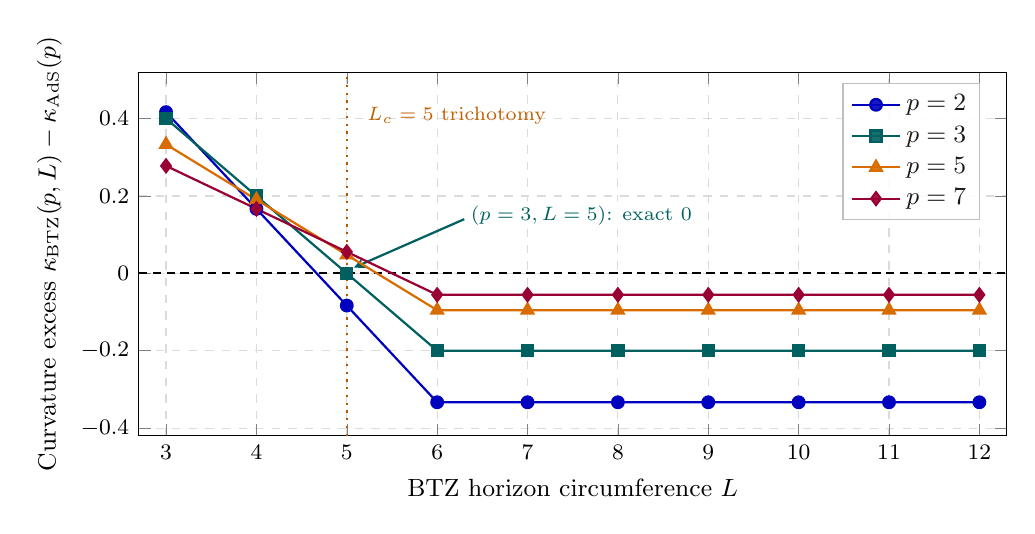
\begin{tikzpicture}
\begin{axis}[
  width=12.6cm,
  height=6.2cm,
  xlabel={BTZ horizon circumference $L$},
  ylabel={Curvature excess $\kappa_{\mathrm{BTZ}}(p, L) - \kappa_{\mathrm{AdS}}(p)$},
  xmin=2.7, xmax=12.3,
  ymin=-0.42, ymax=0.52,
  xtick={3,4,5,6,7,8,9,10,11,12},
  grid=major,
  grid style={dashed, gray!28},
  legend pos=north east,
  legend cell align=left,
  legend style={font=\small, fill=white, fill opacity=0.9, draw=gray!50},
  label style={font=\small},
  tick label style={font=\footnotesize},
]
  % Zero excess reference line
  \addplot[black, thick, densely dashed, forget plot] coordinates {(2.7, 0) (12.3, 0)};
  % Critical circumference L_c = 5 band
  \draw[orange!70!black, dotted, thick] (axis cs:5, -0.42) -- (axis cs:5, 0.52);
  \node[anchor=south west, font=\scriptsize, text=orange!75!black] at (axis cs:5.12, 0.36)
    {$L_c = 5$ trichotomy};
  \draw[->, >=stealth, teal!75!black, thick] (axis cs:6.3, 0.14) -- (axis cs:5.08, 0.015);
  \node[anchor=west, font=\scriptsize, text=teal!75!black, fill=white, fill opacity=0.85, text opacity=1, inner sep=1.5pt] at (axis cs:6.32, 0.15)
    {$(p=3, L=5)$: exact $0$};

  \addplot[color=blue!75!black, thick, mark=*, mark size=2.1pt] coordinates { (3, 0.416667) (4, 0.166667) (5, -0.083333) (6, -0.333333) (7, -0.333333) (8, -0.333333) (9, -0.333333) (10, -0.333333) (11, -0.333333) (12, -0.333333) };
  \addlegendentry{$p = 2$}

  \addplot[color=teal!75!black, thick, mark=square*, mark size=2.0pt] coordinates { (3, 0.400000) (4, 0.200000) (5, 0.000000) (6, -0.200000) (7, -0.200000) (8, -0.200000) (9, -0.200000) (10, -0.200000) (11, -0.200000) (12, -0.200000) };
  \addlegendentry{$p = 3$}

  \addplot[color=orange!85!black, thick, mark=triangle*, mark size=2.4pt] coordinates { (3, 0.333333) (4, 0.190476) (5, 0.047619) (6, -0.095238) (7, -0.095238) (8, -0.095238) (9, -0.095238) (10, -0.095238) (11, -0.095238) (12, -0.095238) };
  \addlegendentry{$p = 5$}

  \addplot[color=purple!80!black, thick, mark=diamond*, mark size=2.3pt] coordinates { (3, 0.277778) (4, 0.166667) (5, 0.055556) (6, -0.055556) (7, -0.055556) (8, -0.055556) (9, -0.055556) (10, -0.055556) (11, -0.055556) (12, -0.055556) };
  \addlegendentry{$p = 7$}
\end{axis}
\end{tikzpicture}
\end{document}
